\section{Motivation} \label{sec:motivation}
%%\vspace{-5pt}
%
In this section, we present the system model of TPCs in Sec.~\ref{sec:motiModel} and propose an image sensing application example to show the software model of programs executed on TPC.
Based on these two models, we analyze the two software and hardware challenges in Sec.~\ref{sec:motiSW} and Sec.~\ref{sec:motiHW}. 

%
\begin{figure}[t]
    \centering
    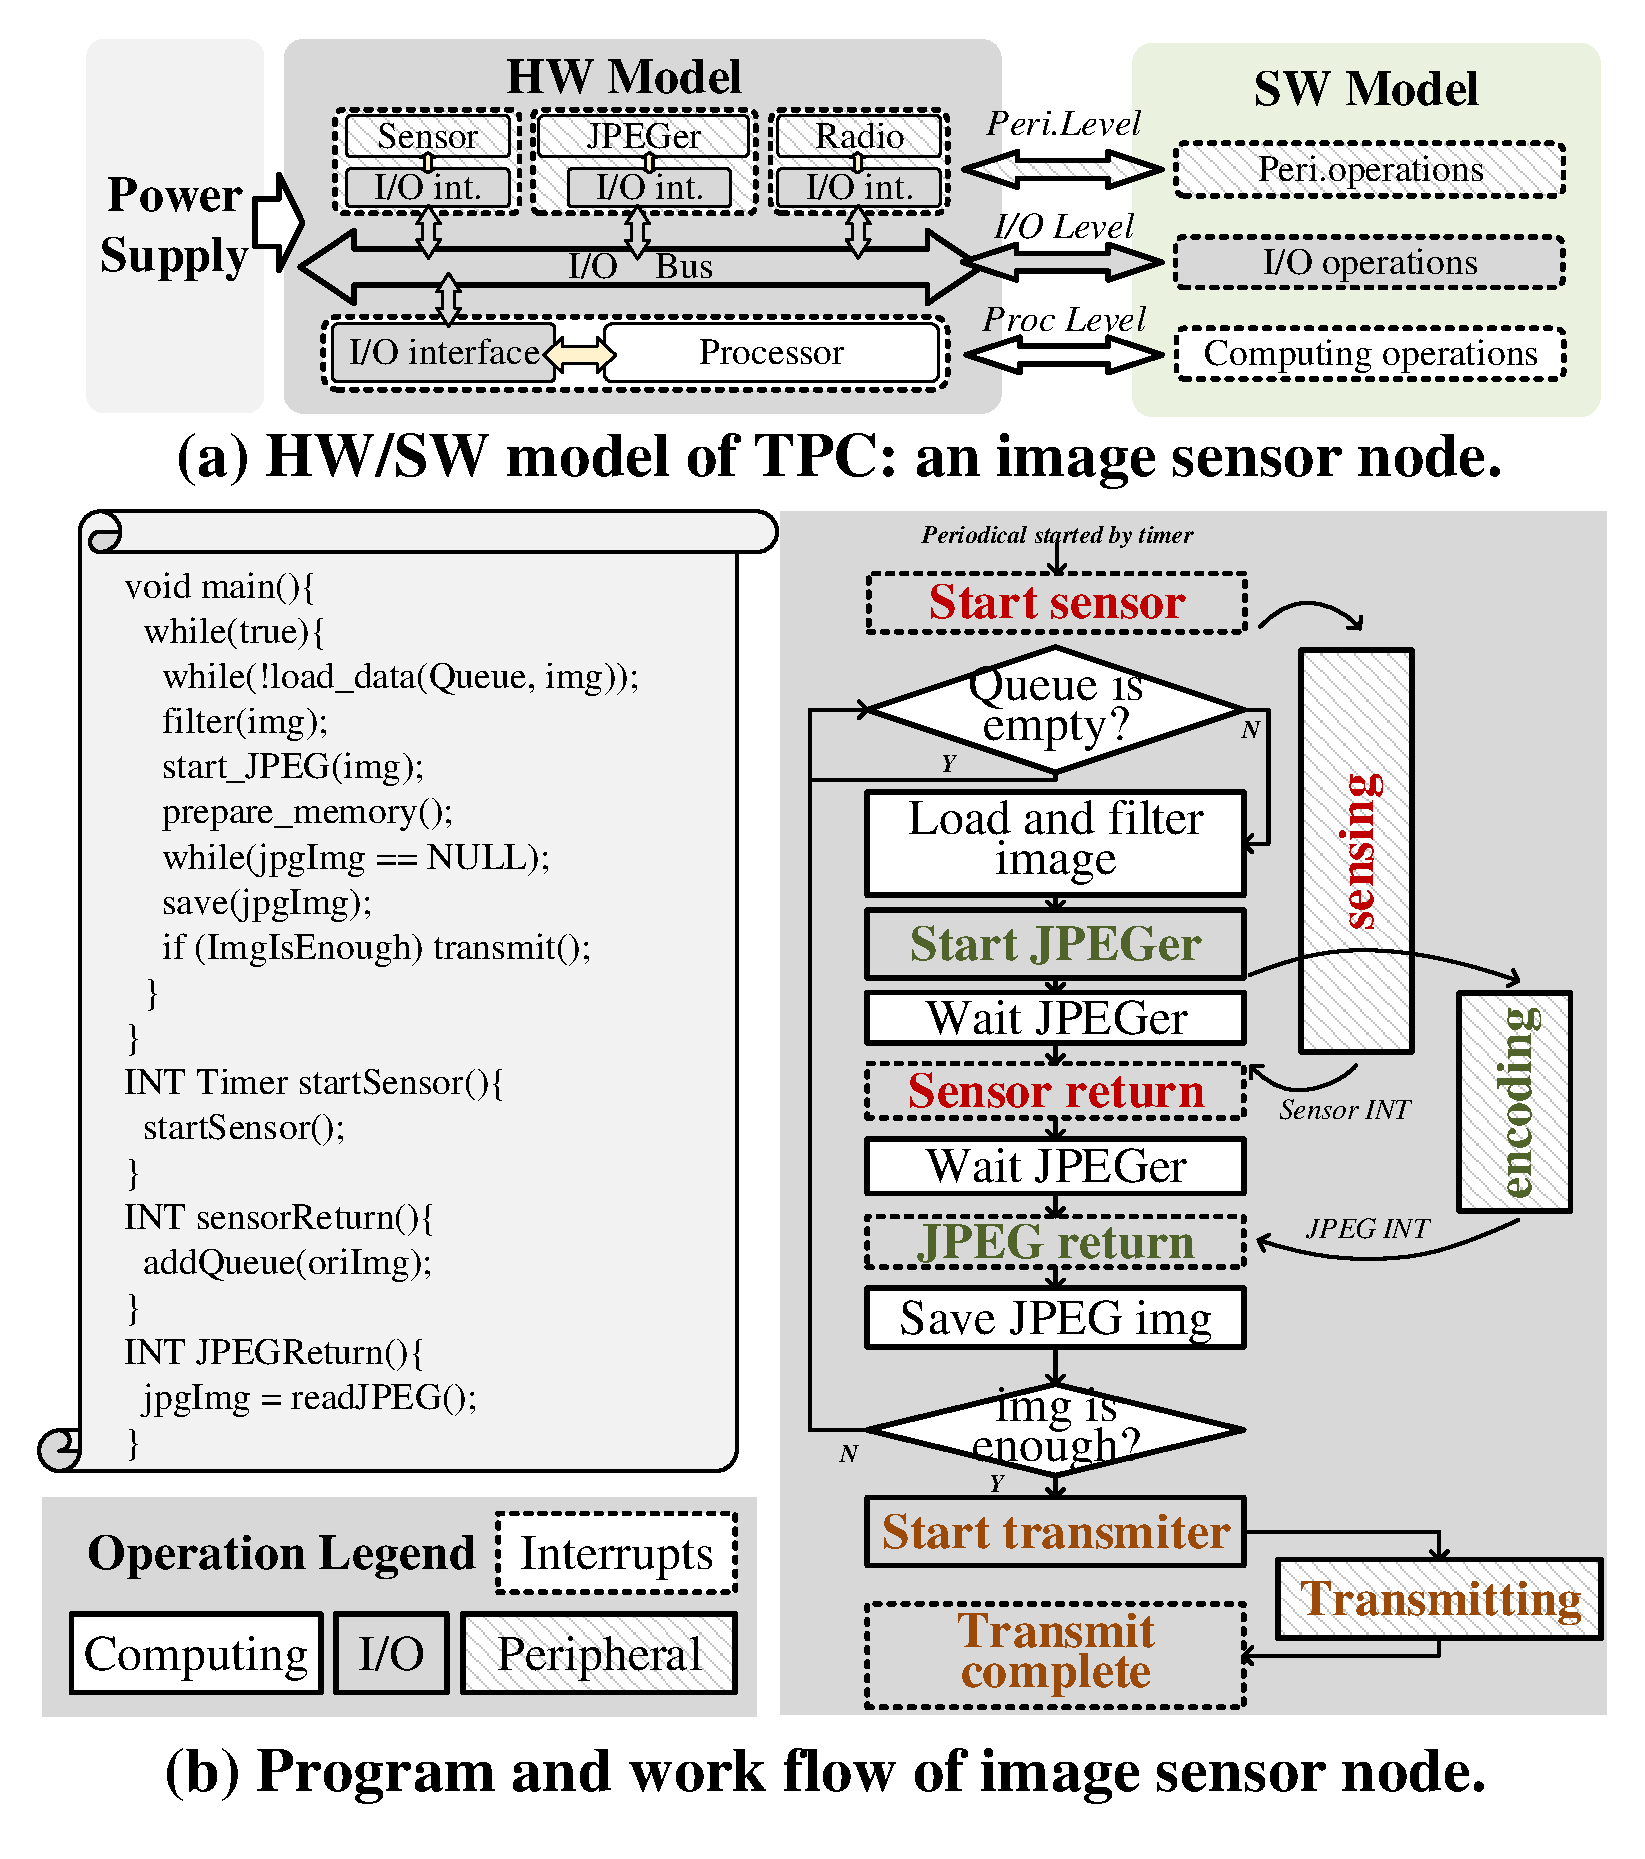
\includegraphics[width=0.47\textwidth]{Fig1_TPCModel.pdf}
    %\vspace{-10pt}
    \caption{An image sensing example used to present the HW/SW model of TPC system.}
    %\vspace{-5pt}
    \label{fig:TPCmodel}
\end{figure}

%\vspace{-5pt}
\subsection{TPC System Model} \label{sec:motiModel}
%\vspace{-5pt}
%
% Problem model and the requirements
Fig.~\ref{fig:TPCmodel} (a) exhibits the hardware structure of a typical TPC and the corresponding three types of operations on each hardware level. 
The sensor node contains a processor, multiple peripherals and the I/O bus to connect these hardware component.
The processor executes \emph{computing operations} and accesses the peripherals via \emph{I/O operations} on the I/O bus.
Peripherals, such as sensor, encoder and radio transceiver, are used to perform specific behaviors, such as sensing, data encoding and transmitting, with \emph{peripheral operations}.
These peripherals can be divided into three categories.
The input-type collects/receives the external information, such as a sensor or a touch screen.
The output-type realizes actuation to outside targets, such as a electromagnetic relay or a wireless transmitter.
The compute-type accelerates computing intensive tasks, such as a JPEG encoder.
Fig.~\ref{fig:TPCmodel} (b) shows the program model of a concurrent peripheral operation.
Before all, a peripheral should be completely initialized via I/O operations by the processor.
Then, the processor will write the start command to the peripheral, also via I/O operation, to start the actuation of the peripheral.
After that, the peripheral concurrently operates a specific peripheral operation and returns an interrupt to announce the processor when completed.
From this procedure, we conclude that, (1) the peripherals requires more preparations to get ready; (2) I/O operations are atomic interacting operations between in the control thread of both processor and peripherals; (3) some peripheral operations are atomic, concurrent operations that only loaded on peripherals.

Fig.~\ref{fig:TPCmodel} (c) shows an image sensing example to explain the model.
The processor maintains two threads, the timer thread and the main thread. 
The timer thread periodically collects and stores the images into buffer.
In the main thread, the processor first initializes all the peripherals.
Then, in the loop of main thread, the processor processes and encodes the images with a JPEG encoder whenever the buffer is not empty.
When the process has stored enough encoded images, the sensor node will transmit all the images back to the server.
In this system, the image sensor is an input-type peripheral that collects outside images.
The radio transmitter is an output-type peripheral to transmit the collected images to the server for further processes.


%
In intermittent power supply scenario, such a system can efficiently recover the processor and the computing operations with existed techniques. 
However, peripherals will lose their states after power failure, which leads to reliability and efficiency issues. 
Based on the type of peripherals, different faults will occur if the devices are not recovered: 
\textbf{1. Input-type Failure} may cause incompleteness and non-determinism. When a sensor loses power, the current collection will be crashed and result is non-deterministic. Even worse, one data lost may jeopardize the integrity of the whole data set in a multi-sensor system.
\textbf{2. Output-type Failure} may leads to large data loss and affect the application procedure. When the transmitter loses power, the current transmitting package as well as the data in peripheral buffer are lost. Moreover, the subsequent processes in the server are affect since none image arrives. Although costly software-level re-transmission can be used in some cases, it may not be feasible for resource-constraint energy-harvesting sensors. 
\textbf{3. Compute-type Failure} may cause fatal disruptions to the program. When the JPEGer loses power, processor cannot receive its returned results and halts all subsequent operations. It may cause system deadlock when program relies on the returned data.
Therefore, a systematical peripheral recovery mechanism is in desperate needs. 

Targeting on this requirement, two challenges arise.
(a) How to design an efficient architecture to recover the execution states in peripherals;
(b) How to devise a reliable checkpointing mechanism for a TPC with multiple peripherals.
The rest of this paper addresses these two challenges.

\subsection{Checkpointing for Concurrent TPC} \label{sec:motiSW}
%\vspace{-5pt}
%
Existing checkpointing strategy faces inefficient and reliability issues in recovering the TPC program where both non-atomic computing operations and atomic concurrent peripherals operations exist.

% static checkpointing
Static checkpointing strategy is safe for atomic operations but not efficient for non-atomic operations.
The red lines in Fig.~\ref{fig:motiRollback} (a) shows the efficiency issue caused by static checkpointing strategies~\cite{ransford2012mementos,Lucia2015,jayakumar2014quickrecall}.
Three execution threads are shown, from top to bottom: the JPEGer thread, the sensor thread and the main thread of the processor.
The program presets checkpoints in position $cp1$, $cp2$ and $cp3$ to protect the atomic operations.
During execution, the program successively starts the sensor and the JPEGer.
Once power failure takes place during the I/O and peripheral operations, the program has to rollback to the complete safe position $cp1$ to restart all the devices which leads to extra waiting time and large rollback overheads.

% dynamic checkpointing
Dynamic checkpointing strategy is efficient for non-atomic computing operations on the processor but not safe for the atomic operations related to peripherals.
The blue lines in Fig.~\ref{fig:motiRollback} (a) shows the reliability issue caused by dynamic checkpointing strategies~\cite{wang20123us,liu2016a,Liu2015Ambient,balsamo2015hibernus}.
When power failure takes, the processor immediately place a checkpoint in position $cp4$.
From $cp4$, the main thread can efficiently continue with not rollback overhead, while all the peripheral devices are left un-recovered. 
Not only the disrupted peripheral operations failed, the peripherals are also left uninitialized which will leads to more errors when the subsequent peripheral-related operations are executed.

%
Both static and the dynamic checkpointing strategies are needed to achieve safe and efficient recovery.
In Fig.~\ref{fig:motiRollback} (b), if the processor is restored to the interrupt position without rollback and all the peripherals are restarted from the static checkpoints before the atomic operations, the recovery overhead can be reduced by 58.5\%.
Therefore, an automatic checkpointing tool supporting a dynamic checkpointing strategy for TPCs with multiple peripheral is needed. 

%   
\begin{figure}[t]
    \centering
    \includegraphics[width=0.48\textwidth]{Fig1_motiRollback}
    %\vspace{-12pt}
    \caption{Challenges using static or dynamic checkpointing strategies in TPC. A hybrid checkpointing framework is needed.}
    %\vspace{-5pt}
    \label{fig:motiRollback}
\end{figure}

%%\vspace{-5pt}
\subsection{Hardware Needs for Peripheral Recovery} \label{sec:motiHW}
%\vspace{-5pt}
%
To support the hybrid checkpointing strategy, we still need hardware modifications based on existing hardware platforms.
Two drawbacks are noticed in the existing hardware platform shown in Fig.~\ref{fig:motiNVM} which contains a nonvolatile processor and sensors.

As is discussed above, NVP is the most efficient dynamic checkpointing strategy which is able to backup and restore (B/R) the processor state within $8\mu s$ once the supply voltage changes across the thresholds. 
However, both the B/R operations are passively triggered by the voltage detector.
NVP do not provide API to support the programmable backup operation for static checkpointing strategy.
Moreover, the processor may trigger unwillingly backup when power failure takes place during an atomic I/O operation in the main thread which will cause consistency problems. 
Therefore, it requires flexible B/R interfaces instead of the passive approach to support the hybrid checkpointing strategy.

% peripheral recover problem: restore and restart
On the other hand, checkpointing and recovering a peripheral also poses challenges.
Fig.~\ref{fig:motiNVM} shows the structure of an image sensor, a typical volatile peripheral.
The sensor contains a digital part using registers to store the states and data, and the analog part to realize the image collection operation.
When power failure takes place during a sensing task, the system has to not only restore the states in the register files, but also restart the analog part to re-execute the uncompleted sensing task to avoid the input-type failure, which is the exact problem beween associate processors and sensors.
 To efficiently and reliably recover concurrent TPCs, the system should support hybrid checkpointing, peripheral status monitor as well as the peripheral restart modules, which are all missing in existing NVPs.
\begin{figure}[t]
    \centering
    \includegraphics[width=0.48\textwidth]{Fig1_motiNVM}
    %\vspace{-15pt}
    \caption{Hardware challenges of multi-device checkpointing. NVP is limited by passive B/R function. Peripherals require efficient reconfigurations and restarts.}
    %\vspace{-5pt}
    \label{fig:motiNVM}
\end{figure}

%To restore the states of the digital parts, existing approaches~\cite{jayakumar2014quickrecall,li2016hw} provides the 'load-and-backup' method.
%To 'load-and-backup' with software methods, the processor has to read the internal registers in the sensor via I/O operations, which is energy hungry and time-consuming.
%Moreover, as the number of peripherals increases, the recovery overhead becomes particularly significant.
% Any proof?
%Li, et al.~\cite{li2016hw} provide hardware based solution by replacing peripheral registers to NVFFs which realizes efficient 'load-and-backup' procedure. 
%But it requires hardware modifications inside the peripherals which is unrealistic considering the variety of peripheral types and producers.
%Therefore, an efficient and general state restoring strategy is needed.
%Furthermore, none existing strategy addresses the problem of restarting an uncompleted peripheral operations. 
%Current systems can only rolling the entire system back to where the broken peripheral operations just started.
%If a hardware module can simply re-execute the peripheral start program and return correctly, the peripheral restart can be more efficient.

%Therefore, to efficiently and reliably recover concurrent TPCs, the enhanced NVP should support hybrid checkpointing, peripheral status monitor as well as the peripheral restart modules, which are all missing in existing NVPs.











